\documentclass[american]{scrartcl}
    \usepackage{babel}
    \usepackage[utf8]{inputenc} 
    \usepackage{csquotes}
    \usepackage{amsmath}
    \usepackage{amssymb}
    \usepackage{graphicx} 
    \usepackage{subfigure}
    \usepackage{mathtools}
    \usepackage{float}
    \usepackage{fancyvrb} % for "\Verb" macro

    
    \setlength{\parindent}{0em}
    \setlength{\parskip}{0.5em}

    % Bibliography and citations
    \usepackage[bibencoding=utf8, style=apa]{biblatex}
    \bibliography{ref}

    
    \title{A model of Cournot Competition with group selection}


    \author{Andrea Titton}
    

% Commands
\newcommand{\set}[1]{\left\{#1\right\}}
\newcommand{\Real}{\mathbb{R}}
\newcommand{\Rat}{\mathbb{Q}}
\newcommand{\abs}[1]{\left\lvert #1 \right\rvert}
\newcommand{\Two}{\mathbf{2}}
\newcommand{\E}{\mathbb{E}}
\newcommand{\citein}[1]{\citeauthor{#1} (\citeyear{#1})}

\begin{document}

% Title

\maketitle

\section{Introduction}


In this short paper I propose to study the dynamics of equilibrium formation in Cournot competition through an evolutionary lens. The aim is to study the formation and sustainability of tacit collusion among firm. I develop a model with local markets competing à la Cournot. Firms evolve in a birth-death process. This can be thought of as firms copying a production technology from the best performing competitor in their own local market, after a certain amount of periods. Here the standard result applies: tacit collusion is stable only for a small number of firms (\cite{Lampart2012}). The model is then extended to encompass group effects, based on the framework by \citein{Akdeniz2020}. In particular, I show how tacit collusion can be sustained for larger oligopolies, as long as competition at a group level (i.e. between local markets) emerges slowly.

\section{Literature review}

In 1838, Antoine Augustin Cournot introduced his famous model of competition over quantities. Since then, the model has served as a theoretical benchmark for pure oligopolistic models in economic theory. In Cournot oligopolies, a discrete number of firms compete by setting quantities of a perfectly substitutable good. In equilibrium, due to symmetry, all firms produce the same quantity and any deviations by producers reduces their own profit.

In proposing the model, Cournot does not address the way in which firms form their strategies. Modern economics relies on rational expectations to justify the symmetric equilibrium solution. More contemporary approaches have derived the model dynamics under limited knowledge (\cite{Bischi2015}) or naive expectations (\cite{Cnovas2008}). All of these approaches lead to equilibria that are unstable as the number of firms increases (Cournot–Theocharis problem).

In order to better model and understand the emergence of such instability I will rely on an evolutionary framework developed by \citein{Akdeniz2020}. The authors analyse the role of group selection in the emergence of cooperation. As in previous models, defection gives a fitness advantage at an individual level (within groups) but a disadvantage at a group level (across groups). Furthermore, groups do not compete globally but only with neighboring groups. The authors show how local competition among groups has strong implications for the emergence of cooperation.

\section{Theoretical formulation}

As in \citein{Akdeniz2020}, the game is played within groups (hereafter, local markets). Firms compete locally à la Cournot. Each turn there is a probability of a global event where two markets merge (i.e. they form one larger local market). This mechanisms is different from that of group reproduction in the baseline framework (\cite{Akdeniz2020}) because it represents a more realistic assumption in the case of firms competing and it better encodes the tradeoffs between tacit collusion and competition.

\subsection{Notation}

Any variable $x^{(i)}_t$ is indexed such that the superscript refers to the individual and the subscript to time.

\subsection{Local markets}

Local markets are composed by $N$ firms, indexed by $i$, that can choose a production quantity $q^{(i)} \in \Sigma \subset \Rat_+$. Firms face linear demand,

\begin{equation}
    p(Q) = p\left(q^{(1)}, q^{(2)},  \ldots, q^{(N)} \right) = a - b \cdot \sum^{N}_{i=1} q^{(i)}
\end{equation}

where $Q$ is the vector of quantities and $a$ and $b$ are chosen for normalization purposes. The normalization is introduced to guarantee that the ``standard'' Cournot equilibrium is in the interior of $\Sigma$. Furthermore, firms face no fixed nor marginal costs. All of these assumptions can be easily relaxed to allow for non-linear demand, entry costs, and marginal costs. The symmetric Nash equilibrium of the game is (Appendix \ref{A:cournot}),

\begin{equation} \label{equilib}
    \bar{q}= \frac{a}{b \cdot (N+1)}
\end{equation}

The model evolves in discrete time $t \in \set{0, 1, \ldots T}$ and firms are assumed to enter the market playing a random draw from the strategy set,  $q^{(i)}_0 \sim U(\Sigma)$. In every period each company realizes a payoff, $\Pi^{(i)}_t = p(Q_t) \cdot q^{(i)}_t$. I assume that firms reproduce in a birth-death process. That is, each turn, with a probability proportional to its payoffs, a firm is picked to reproduce and, with uniform probability, a firm is picked to die. To account for negative fitness (i.e. negative profits), the probability weights assigned to each firm are a softmax mapping of the profits. In particular, the probability of a strategy, say $\sigma \in \Sigma$ played by $n$ firms, being picked for reproduction is,

\begin{equation}
    \frac{n \cdot \exp(P(Q_t) \cdot \sigma)}{\sum_{i} \exp(P(Q_t) \cdot q^{(i)})}.
\end{equation}



This modelling choice is justified in the context of oligopolies where firms copy other firms' production quantities in case the competitor is experiencing better profits. This arises for example in the airline industry, where capacity (number of flights) has to be planned \textit{ex-ante} to comply with regulations. Furthermore, these are markets with high barriers to entry (fixed $N$), long-term investment commitments (randomness in the birth-death process), and common tacit collusion.

\subsection{Global market}

In the model, there are $M$ local markets and each local market is linked to two other neighboring markets, thus forming a cycle (as in \cite{Akdeniz2020}). With arrival rate $\rho$, a market is chosen at random, with probability $1 / M$, and is merged with its best performing neighbor. This mechanisms is illustrated in Figure \ref{fig:diagram}.

This choice arises assuming that highly profitable local markets will be invaded by neighboring firms. For illustration purposes, consider again the airline industry example. Routes were airline are colluding, generate higher profits and, as a consequence, are more likely to be invaded by neighboring airlines. On the other hand, regardless of how high the profits are, non-neighboring airlines face high barriers to enter the market. In this way tacit collusion, on the one hand, pushes up payoffs and, on the other hand, it increases the likelihood of a neighboring entry.



\begin{center}
    \begin{figure}[H]
        \center
        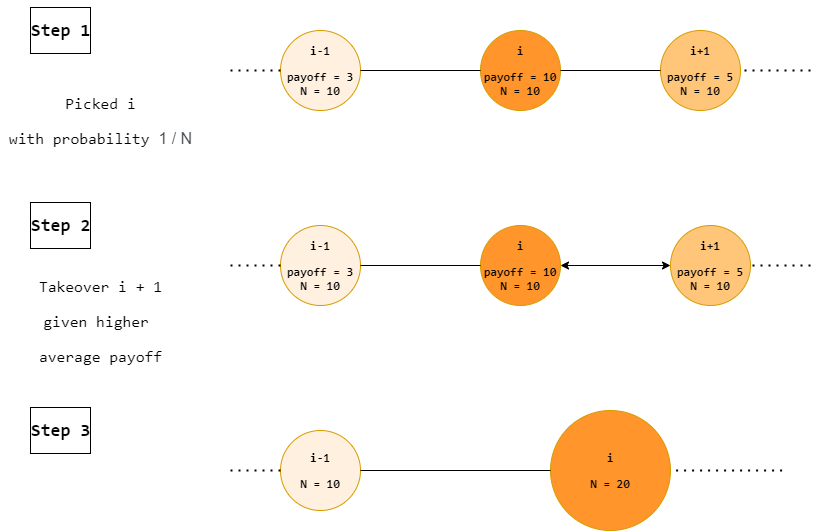
\includegraphics[width=0.8\textwidth]{../plots/step_group.png}
        \caption{Diagram illustrating the takeover in the global market}
        \label{fig:diagram}
    \end{figure}
\end{center}


\section{Simulation}

To reproduce the simulation see Appendix \ref{A:code}.

In the simulations I set $\Sigma = \set{1, 2, \ldots, 10}$, $a = (N + 1) \cdot 5$, and $b = 1$, such that equation (\ref{equilib}) yields,

\begin{equation}
    \bar{q} = 5
\end{equation}

\subsection{Local market}

First we can focus on a simulation of a local market, without group effects (i.e. no global markets). In particular here we look at the evolution of quantities and prices, first with a concentrated market ($N = 5$) and then with a competitive market ($N = 20$). The values of $N$ are set to these values heuristically based on the simulation results.

Figure \ref{fig:small_local} shows a quantity heat map for one of the runs, with $T = 200$, in the case of a concentrated market. Each row represents a firm in the market and each column a time step. Darker colors are associated with smaller quantities. As expected, tacit collusion occurs very quickly as all firms synchronize to a low quantity.

\begin{center}
    \begin{figure}[H]
        \center
        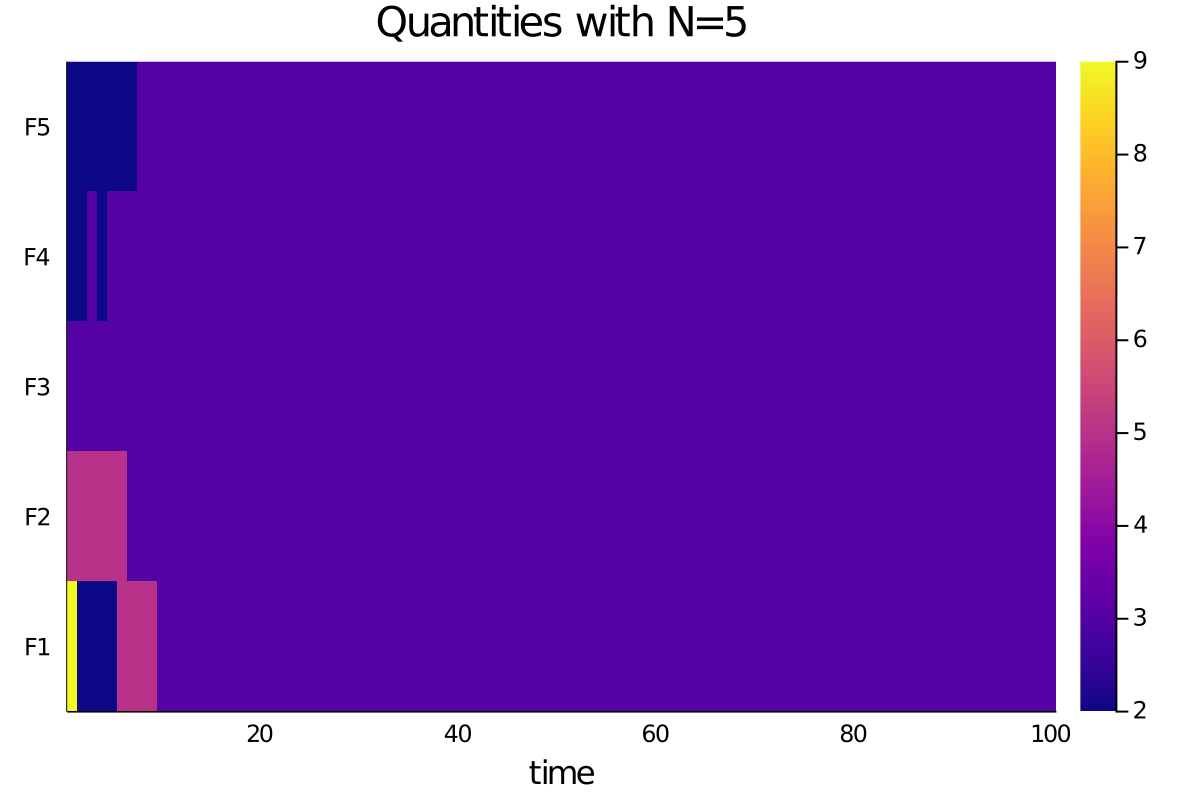
\includegraphics[width=0.8\textwidth]{../plots/local/q_group_heat_5.png}
        \caption{Quantity evolution in a concentrated market}
        \label{fig:small_local}
    \end{figure}
\end{center}

Figure \ref{fig:price_small_local} displays the price evolution $p(Q_t)$ of $150$ simulations with concentrated markets. All simulations display tacit collusion but also high path dependence of the equilibrium price. This is expected as the strategy set is restricted to the initial sample of strategies $Q_0 \sim U(\Sigma)$, hence if enough firms start off producing a quantity above $\bar{q}$ which yields $p(Q_0) \approx 0$, firms who produce the highest quantity have greater payoffs and hence the price will be driven further down.

\begin{center}
    \begin{figure}[H]
        \center
        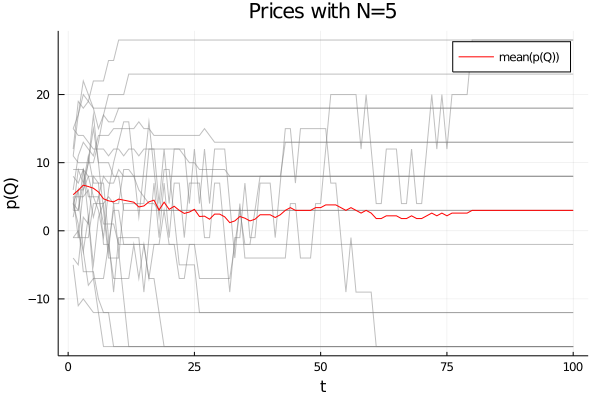
\includegraphics[width=0.8\textwidth]{../plots/local/p_group_5.png}
        \caption{Price evolution in a concentrated market}
        \label{fig:price_small_local}
    \end{figure}
\end{center}

If we turn our attention to a highly competitive markets and we repeat the exercise, the dynamics change drastically. In particular, Figure \ref{fig:large_local} shows the evolution of strategies of a single run. Here firms fail to collude and prices tend towards the equilibrium.

\begin{center}
    \begin{figure}[H]
        \center
        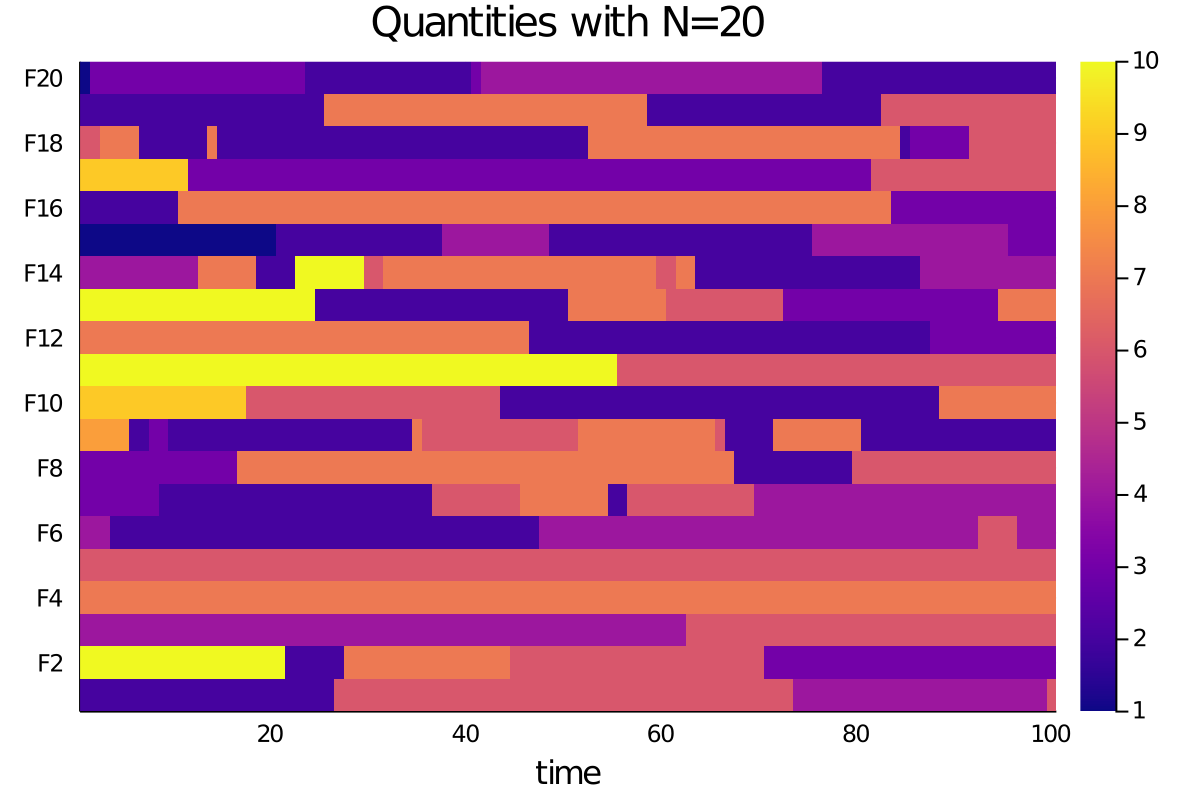
\includegraphics[width=0.8\textwidth]{../plots/local/q_group_heat_20.png}
        \caption{Quantity evolution in a competitive market}
        \label{fig:large_local}
    \end{figure}
\end{center}

The lack of collusion can be seen more clearly in the 150 simulations run of price in Figure \ref{fig:price_large_local}.

\begin{center}
    \begin{figure}[H]
        \center
        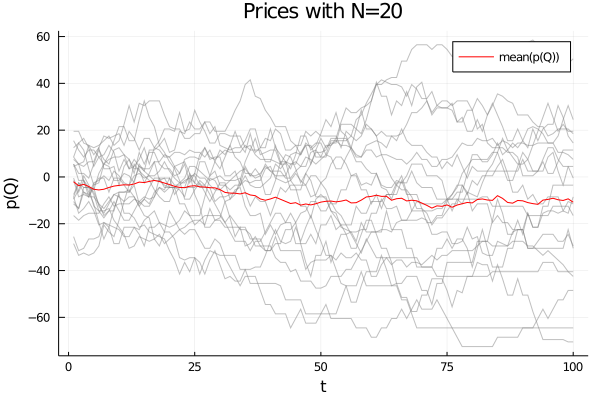
\includegraphics[width=0.8\textwidth]{../plots/local/p_group_20.png}
        \caption{Price evolution in a competitive market}
        \label{fig:price_large_local}
    \end{figure}
\end{center}

\subsection{Global markets}

In order to study the effect of groups on the equilibria of the game we first look at a simple simulation run with, as before, $N = 5$ and $M = 4$. In Figure \ref{fig:small_avg}, two lines, representing the average quantity in each group, are plotted with the same color if in that period the local markets are merged. Already from a single run we can see how tacit collusion can be sustained in larger groups, if these arise from smaller prior groups which were in a tacit collusive equilibrium. In fact the previous simulation with $N = 20$ and no group effects does not sustain collusion but $M = 4$ and $N = 5$ does (note that $M\cdot N = 20$ is the long run size of the group as all groups will be merged).

\begin{figure}[H]
    \center
    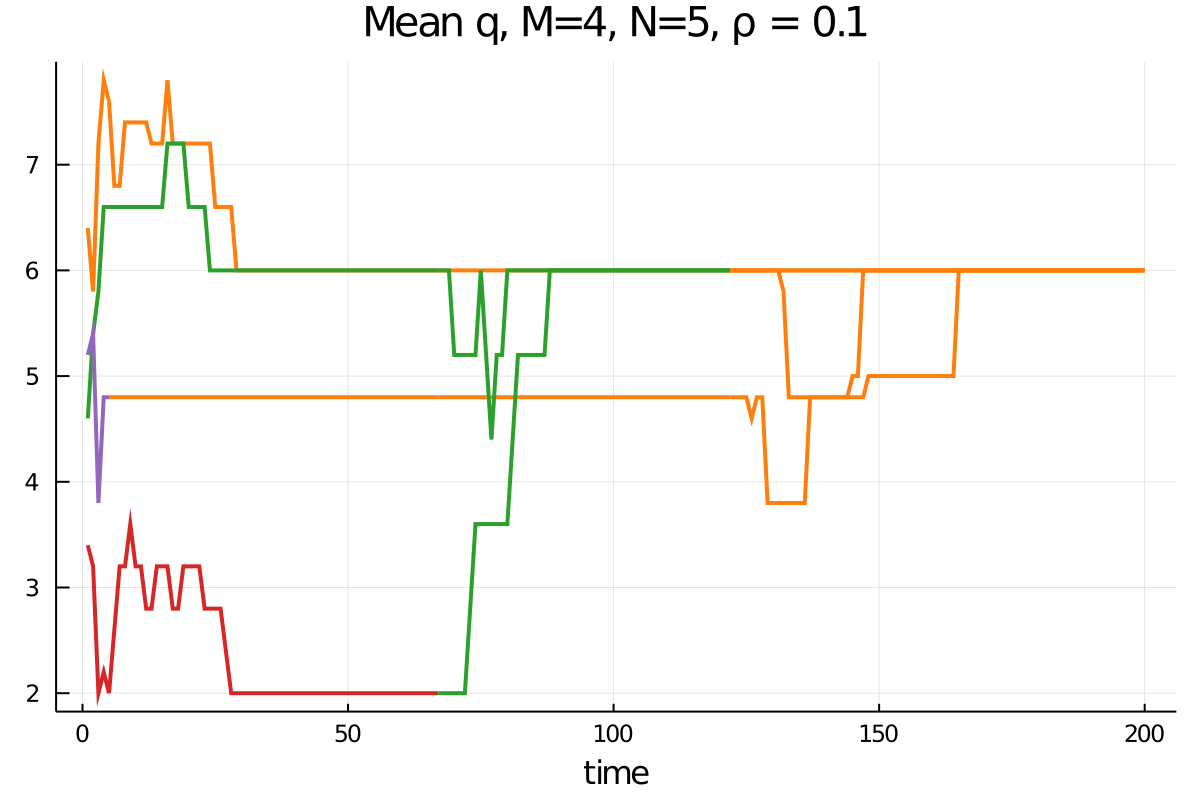
\includegraphics[width=0.8\textwidth]{../plots/group/q_group_4-5.png}
    \caption{Average quantities with $4$ markets of size $5$}
    \label{fig:small_avg}
\end{figure}

The same dynamics can be seen by plotting the profits over this run (Figure \ref{fig:small_avg_profit}).

\begin{figure}[H]
    \center
    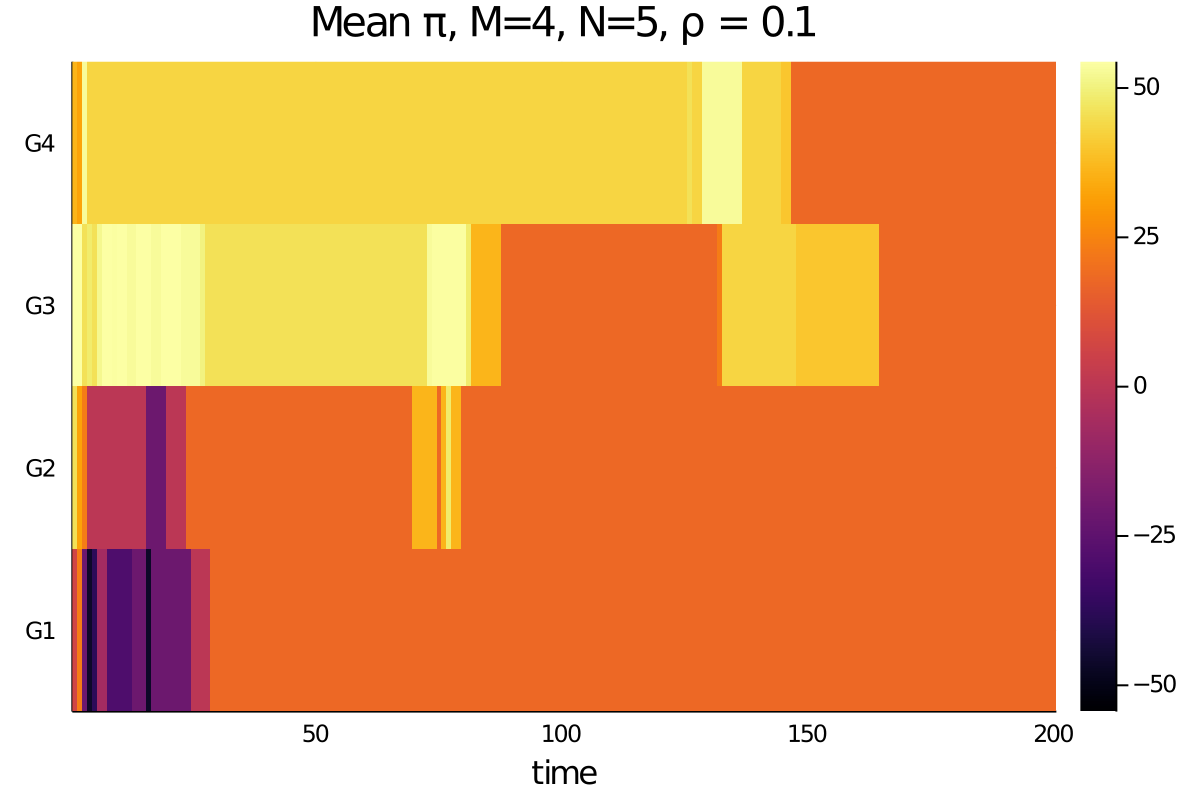
\includegraphics[width=0.8\textwidth]{../plots/group/pi_group_4-5.png}
    \caption{Profits with $4$ markets of size $5$}
    \label{fig:small_avg_profit}
\end{figure}

Given this result it is clear that group effects have implications for the sustainability of tacit collusion. In particular, the expected local market size (Equation \ref{market_size}, derived in Appendix \ref{A:exp_size}) at each time step, $\E[N_t]$, depends on both the takeover frequency and the number of groups $M$,

\begin{equation} \label{market_size}
    \E[N_t] = (1 - \rho)^t \cdot N + \rho \cdot \sum^{t-1}_{i = 0} (1 - \rho)^{i} \cdot \frac{N \cdot M}{M - (t - i)}.
\end{equation}

This function, plotted for $M = 10$ and $N = 5$ can be seen in Figure \ref{fig:size}.


\begin{figure}[H]
    \center
    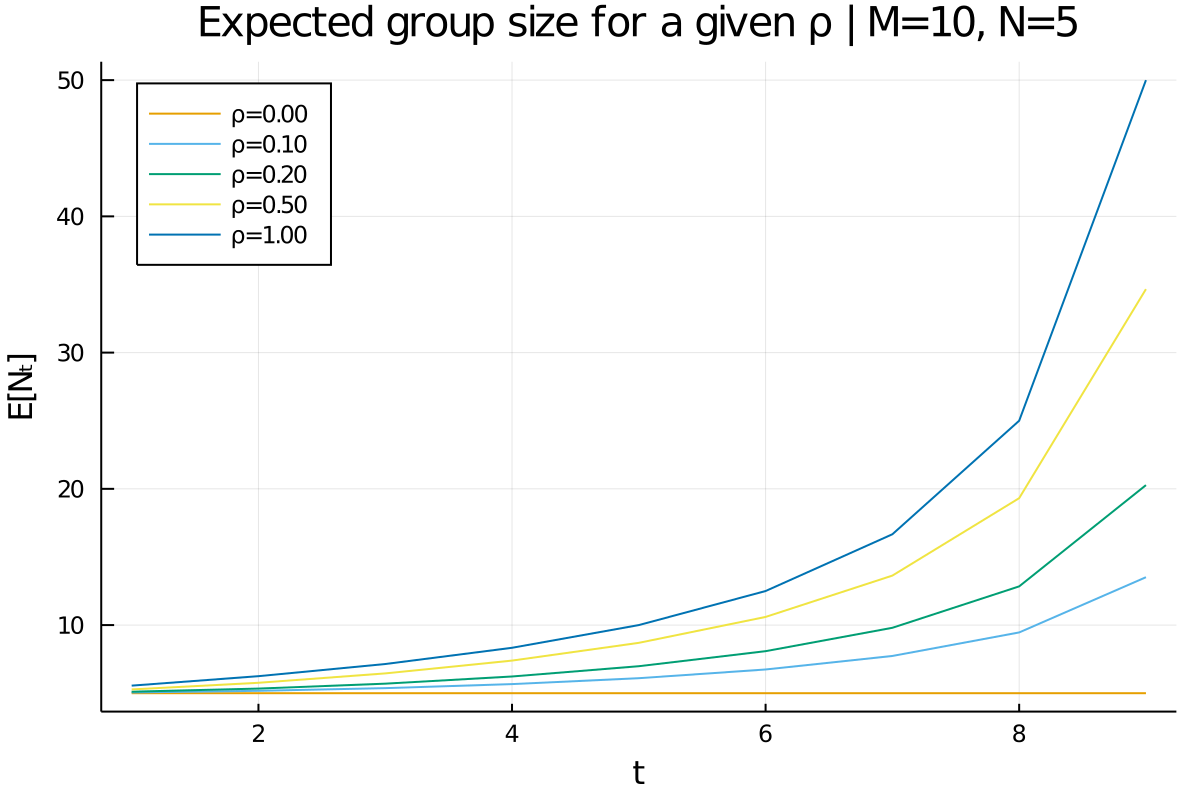
\includegraphics[width=0.95\textwidth]{../plots/expected.png}
    \caption{Expected market size for different $\rho$s.}
    \label{fig:size}
\end{figure}

Despite having derived $\E[N_t]$, the relationship between $\rho$ and tacit collusion is more subtle and depends on the whole distribution of $N_t$ and not only its expected value. To study this I employ a Monte-carlo simulation. Given $M = 40$, for each $N \in \set{3, 4, \ldots, 40}$ and $\rho \in \set{0, \frac{1}{100},\frac{2}{100}, \ldots, 1}$, I compute $200$ simulations of length $T = 200$ of the model. I then look at the variance of the quantity in each group at the end of the 200 periods. If the variance is 0 we have evidence of tacit collusion since each firm is playing the same quantity. Finally, I compute the average variance across groups and simulations. The result of this exercise is presented in Figure \ref{fig:frontier} where $N$ is plotted on the $x$-axis, $\rho$ on the $y$-axis, and the intensity of the color is the average variance of the strategy. Hence dark colors represent common tacit collusion. The simulation clearly shows that low frequencies of mergers renders tacit collusion sustainable with larger groups.

\begin{figure}[H]
    \center
    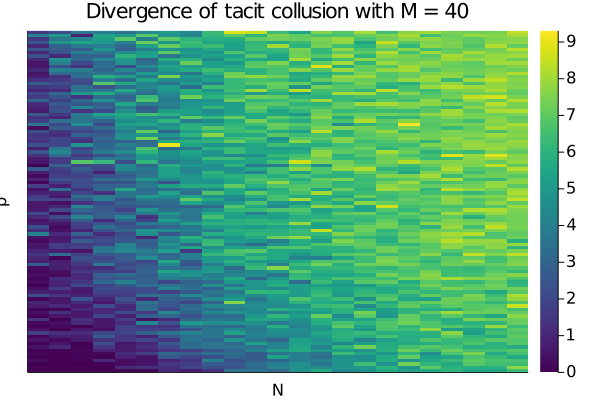
\includegraphics[width=0.95\textwidth]{../plots/global/small_convergence_restr.png}
    \caption{Collusion frontier of $N \in \set{3, 4, \ldots, 40}$ and $\rho \in [0, 1]$ }
    \label{fig:frontier}
\end{figure}

\section{Conclusions}

In this short paper I present a tentative analysis of the dynamics of an oligopolistic market with Cournot competition and group structure. In particular I show how, ceteris paribus, tacit collusion can be sustained for larger market sizes in the presence of slowly merging local markets. The analysis is by no means exhaustive. In particular it lacks an analytical derivation of the relationship between $M$ and $\rho$, and the instability of tacit collusion. Nevertheless, I believe that introducing group structure and evolutionary dynamics can help greatly in modelling the dynamical aspects of Cournot games. This yields a new point of view and can serve as a stepping stone to explain the presence of tacit collusion in apparently competitive markets.

\newpage
% Bibliography
\nocite{*}
\pagenumbering{gobble} % stop page numbering
\printbibliography

\newpage
\appendix

\section{Cournot equilibrium} \label{A:cournot}

Let $q^{(-i)} = Q \setminus \set{i}$. Then the payoff function of firm $i$ is,

\begin{equation*}
    \Pi\left(q^{(i)}, q^{(-i)} \right) = q^{(i)} \cdot p(Q)
\end{equation*}

Then the best response strategy, under ration expectations, is,

\begin{equation*}
    \begin{split}
        \bar{q} = \arg\max_{q} \Pi\left(q, q^{(-i)} \right),
    \end{split}
\end{equation*}

which yields the first order condition,

\begin{equation*}
    \bar{q} \cdot \frac{ \partial p}{\partial q}\left(\bar{q}, q^{(-1)}\right) + p\left(\bar{q}, q^{(-1)}\right) = 0.
\end{equation*}

With a linear demand function, by symmetry it is straight forward to show that,

\begin{equation*}
    \bar{q} = \frac{a}{b \cdot (N+1)}
\end{equation*}

\section{Expected size of global markets} \label{A:exp_size}

Consider the case of $\rho = 1$. Then the expected size of a group sampled at time $t$ is,

\begin{equation*}
    \begin{split}
        \E[N_0 \vert \ \rho = 1] &= N \cdot \frac{M}{M} \\
        \E[N_1 \vert \ \rho = 1] &=  N \cdot \frac{M}{M-1}  \\
        \E[N_2 \vert \ \rho = 1] &=  \frac{1}{M-1} \cdot \left[ \frac{3N + (M-3) \cdot N}{M-2} \right] + \frac{M-2}{M-1} \cdot \left[ \frac{2 \cdot 2N + (M-4) \cdot N}{M-2} \right] \\ &= N \cdot \frac{M}{M-2} \\
        &\vdots \\
        &= N \cdot \frac{M}{M-t}
    \end{split}
\end{equation*}

This result can intuitively be derived by noticing that the total number of firms across markets is constant at $N \cdot M$ but the number of group decreases by $1$ at every merger. Now, for an arbitrary $\rho$ it is trivial to see that $\E[N_0] = N$. Furthermore,

\begin{equation*}
    \begin{split}
        \E[N_t] &= \underbrace{(1 - \rho) \cdot \E[N_{t-1}]}_{\text{no event}} + \underbrace{\rho \cdot \frac{N \cdot M}{M-t}}_{\text{merger event}} \\
        &= (1 - \rho) \cdot \left[ (1 - \rho) \cdot \E[N_{t-2}] + \rho \cdot \frac{N \cdot M}{M - (t-1)} \right] + \rho \cdot \frac{N \cdot M}{M-t} \\
        &=(1 - \rho)^2 \cdot  \E[N_{t-2}] + \rho \cdot (1 - \rho) \cdot \frac{N \cdot M}{M - (t - 1)} + \rho \cdot \frac{N\cdot M}{M-t} \\
        &= (1 - \rho)^3 \cdot  \E[N_{t-3}] + \rho \cdot (1 - \rho)^2 \cdot \frac{N \cdot M}{M - (t - 2)} + \rho \cdot (1 - \rho) \cdot \frac{N \cdot M}{M - (t - 1)} + \rho \cdot \frac{N\cdot M}{M-t}  \\
        &\vdots \\
        &= (1 - \rho)^t \cdot \underbrace{\E[N_0]}_{N} + \rho \cdot \sum^{t-1}_{i = 0} (1 - \rho)^{i} \cdot \frac{N \cdot M}{M - (t - i)}
    \end{split}
\end{equation*}


\section{Simulation code} \label{A:code}

The code can be found at,

\begin{verbatim}
    github.com/NoFishLikeIan/tinbergen/tree/master/code/evolutionary
\end{verbatim}

The simulation requires \verb+Julia v.1.5.x > +. A simulation to produce all graphs is available as,

\begin{verbatim}
    julia main.jl
\end{verbatim}

and to run the coalition size simulation as,

\begin{verbatim}
    julia coalitionsize.jl
\end{verbatim}




\end{document}